\noindent {\bf Requirements/Assumptions}: this recipe assumes the availability of a single head node
{\em master}, and four {\em compute} nodes. The {\em master} node is
provisioned with \baseOS{} and is subsequently configured to provision the
remaining {\em compute} nodes with Warewulf in a stateless configuration. For
power management, we assume that the compute node BMCs are available via IPMI
from the chosen master host. For file systems, we assume that the chosen master
server will host an \NFS{} file system that is made available to the compute
nodes. Installation information is also discussed to optionally include
a \Lustre{} file system mount and in this case, the \Lustre{} file system is
assumed to exist previously.
% We
% assume that the an external \$HOME file system is available for use on both the master
% and compute nodes (via either \NFS{} or \Lustre{}), and that compute node BMCs are
% available via IPMI from the chosen master host.

\begin{figure}[hb]
\center
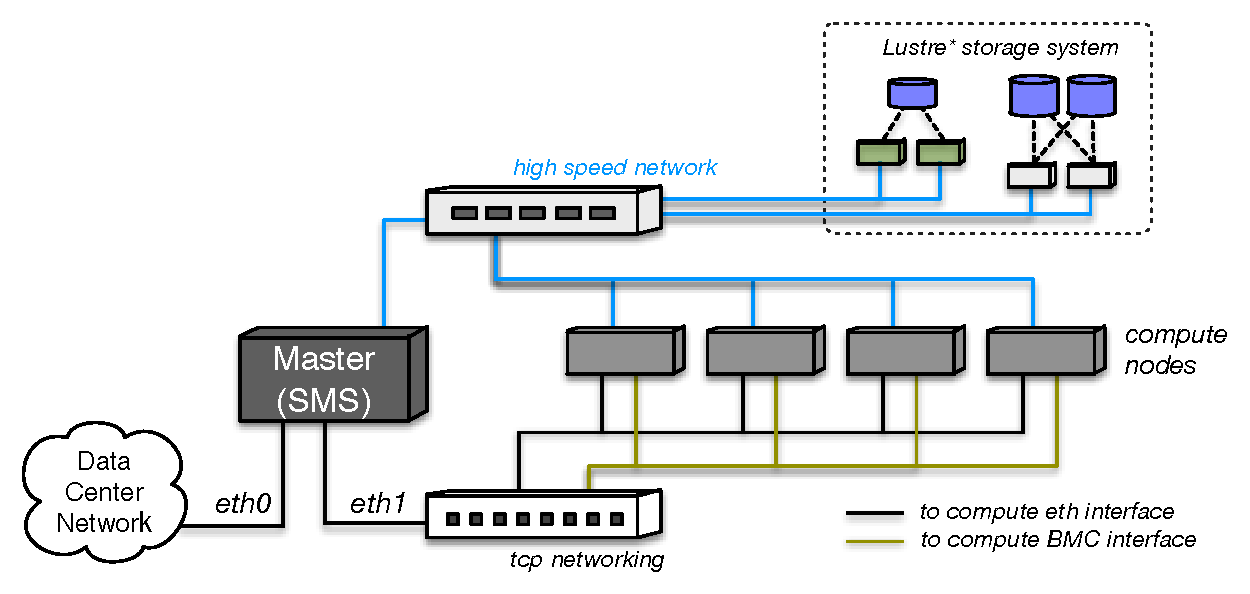
\includegraphics[width=0.8\linewidth]{fsp-arch-small.pdf}
\vspace*{-0.1cm}
\caption{Overview of physical cluster for architecture.}
\end{figure}


How about this?
